\documentclass{article}
\usepackage{tikz, comment}
\usepackage{pifont}
\usepackage{fontspec}
\usetikzlibrary{arrows, decorations.markings, decorations.pathreplacing}
\begin{comment}
:Title: Not defined yet
:Tags: area using polar coordinates, polar integral formula ;sine, sin ;sohcahtoa;cis;polar form of a complex number
:Prob: 0.3601;0.3271;0.3152;0.2945;0.2848
:Slug: No name yet

Description Here.........
\end{comment}
\begin{document}\centering

\newcommand{\AxisRotator}[1][rotate=0]{%
\tikz [x=0.25cm,y=0.60cm,line width=.2ex,-stealth,#1] \draw (0,0) arc (-165:165:1 and 1);%
}

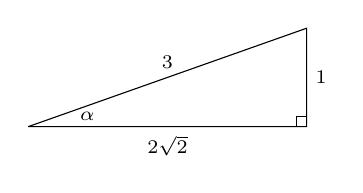
\begin{tikzpicture}[>=latex,xscale=.5*2.5, yscale=.5*2.5][font=\sf\small]

%\draw[xstep=1cm,ystep=1cm,color=gray!80] (0, -1) grid (8, 8);

\foreach \x in {}
\draw (\x,2pt/1.5) -- (\x,-2pt/1.5)
node[anchor=north] {\tiny$\x$}
;
\foreach \x in {}
\draw (\x,2pt) -- (\x,-2pt)
node[anchor=south] {\tiny$\x$}
;
\foreach \y in {}
\draw (-2pt,\y) -- (2pt,\y)
node[anchor=east] {\tiny $\y$}
;

\draw (0, 0)--++({sqrt(8)}, 0)
node[black, below, midway, pos=0.5, xshift=0, yshift=0, scale=1]{\scriptsize $2\sqrt 2$}
--++(0, 1)
node[black, right, midway, pos=0.5, xshift=0, yshift=0, scale=1]{\scriptsize $1$}
--++({-sqrt(8)},-1)
node[black, above, midway, pos=0.5, xshift=0, yshift=0, scale=1]{\scriptsize $3$};

\node at (0.6, 0.1) {\scriptsize $\alpha$};

\draw ({sqrt(8)-0.1}, 0)--++(0,0.1)--++(0.1,0);

\end{tikzpicture}
\end{document}